\documentclass[10pt,twocolumn,letterpaper]{article}


\usepackage{cvpr}
\usepackage{times}
\usepackage{epsfig}
\usepackage{graphicx}
\usepackage{amsmath}
\usepackage{amssymb}
\usepackage{fixltx2e}
\usepackage{dblfloatfix}


% Include other packages here, before hyperref.


% If you comment hyperref and then uncomment it, you should delete
% egpaper.aux before re-running latex.  (Or just hit 'q' on the first latex
% run, let it finish, and you should be clear).
\usepackage[breaklinks=true,bookmarks=false]{hyperref}


\cvprfinalcopy % *** Uncomment this line for the final submission


\def\cvprPaperID{****} % *** Enter the CVPR Paper ID here
\def\httilde{\mbox{\tt\raisebox{-.5ex}{\symbol{126}}}}


% Pages are numbered in submission mode, and unnumbered in camera-ready
%\ifcvprfinal\pagestyle{empty}\fi
\setcounter{page}{1}
\begin{document}


%%%%%%%%% TITLE
\title{Visualizing sub-networks in deep convolutional neural networks}


\author{Spandan Madan\\
Harvard University\\
Cambridge, MA 02138\\
{\tt\small smadan@mit.edu}
\and
Shantanu Jain\\
Massachusetts Institute of Technology\\
Cambridge, MA 02139\\
{\tt\small jains@mit.edu}
% For a paper whose authors are all at the same institution,
% omit the following lines up until the closing ``}''.
% Additional authors and addresses can be added with ``\and'',
% just like the second author.
% To save space, use either the email address or home page, not both
\and
Matthew Tancik\\
Massachusetts Institute of Technology\\
Cambridge, MA 02139\\
{\tt\small tancik@mit.edu}
}


\maketitle
%\thispagestyle{empty}


%%%%%%%%% ABSTRACT
\begin{abstract}
  Deep convolutional neural networks have recently demonstrated great success in computer vision problems. While there have been several efforts to understand how these networks work, we are still far from truth. Moreover, most of the exploratory work done has been in the domain of understanding object and scene detectors. Our motivation is two fold - expanding the domain of standard network visualization techniques to the domain of text recognition, and most importantly, proposing new general purpose visualization pipelines which rely on identifying subnetworks which may be performing a high level function, as opposed to the standard per unit visualization. Identifying meaningful substructures in the network can prove to be useful in both understanding how these large networks work, and in optimizing network architecture and training paradigms.
\end{abstract}


%%%%%%%%% BODY TEXT
\section{Introduction}
Convolutional neural networks have experienced unprecedented success in various computer vision tasks recently.  With applications ranging from object detection \cite{krizhevsky2012imagenet}, segmentation \cite{DBLP:journals/corr/GirshickDDM13}, text recognition \cite{Jaderberg14d}, CNN's have quickly become a staple in the computer vision community. Their success can be partially attributed to the networks ability to learn invariants in the high dimensional space \cite{bengio2013representation}. While the idea was first introduced by LeCun et al in the early 1990s, several factors have contributed to their unprecedented success - (i) the availability of much larger training sets with millions of labeled samples, (ii) powerful GPUs and more computational horsepower making it possible to train networks larger than ever, and (iii) better training strategies for regularization using dropout \cite{wan2013regularization} and batch normalization \cite{ioffe2015batch}.


Despite their successes, CNNs are largely black boxes, with limited understanding about what they have learned, and how they handle different kinds of input. Without a firm understanding of what the CNN is doing, it becomes difficult to improve and optimize network topologies and techniques without trial and error. While there are a number of papers working on visualizing the internal representation of hidden layers, most of them have focused on per-unit visualizations \cite{yosinski2015understanding,mahendran2015understanding,zhou2014object}. Moreover, most of this work has been done on models trained for the task of object and scene recognition. We take this one step further by extending these existing techniques to the domain of text recognition, which has seen significant success with CNNs \cite{Jaderberg14,Jaderberg14c,Jaderberg14d}. As text is inherently synthetic data, and because we work with a synthetic dataset, it gives us the power to address aspects which may be missing in object/scene datasets. In particular, transformations such as scaling, rotation, and translation have not been visualized in networks before.


Further, we believe that instead of using the per-unit visualizations that are popular in literature these days, it might be helpful to visualize substructures in the network which contribute to learning a high level feature. To address this, our work explores different visualization techniques which aim to identify a sub-network, or a path of information flow in the network which may be related closely with either (i) A particular kind of input image, or (ii) A particular kind of output class. We propose a method akin to how a neurologist would use functional magnetic resonance imaging to map out the brain by mapping out regions of activity while performing specific tasks \cite{friston1998event}. We experimentally demonstrate the our visualization techniques for transformations by using a network trained to read text in the wild.


The motivation behind mapping substructures to the high level features stems from both a scientific and applied standpoint. Such maps could help unravel black-box like CNNs to understand their functionality, and may even help optimize network design and training.


\subsection{Main Contributions}
Our contributions are three-fold:
\begin{enumerate}
\item We extend standard visualization techniques to a new domain - a state of the art text recognition network.


\item We propose visualization techniques which help identify sub-networks preferentially activated by a certain kind of input images.


\item We demonstrated our proposed visualization techniques in the context of text recognition.
\end{enumerate}


\subsection{Main Limitations}
Our techniques can be useful for visualizing the network if the structures of interest exist in the convolutional layers. If instead they exist in the fully connected layers, not much useful information can be extracted. More generally these visualization techniques can only supplement, not replace prior techniques. Actionable information correlates highly with the type of transformations and networks being explored. Unfortunately predicting when the actionable information will exist is difficult and unsolved. Regardless this is an issue that is inherent in visualization and debugging tools.


\section{Related Work}
\subsection{CNN Visualization}
With the advent of CNNs, there has been a growing interest in the both the computer vision and the deep learning community to understand how these models work. Most recent works build on creating natural pre-images \cite{DBLP:journals/corr/MahendranV15} that maximally activate certain nodes of the network, or obtaining saliency maps from these networks using techniques like deconvolution \cite{DBLP:journals/corr/ZeilerF13} and
projecting back fully connected layers \cite{DBLP:journals/corr/SimonyanVZ13}. However, most work in this field has been limited to the domain of object and scene detectors, and use a single neuron as the basis of the visualization, identifying exemplar neurons that strongly correspond to high level features \cite{zhou2014object,DBLP:journals/corr/GirshickDDM13,DBLP:journals/corr/MahendranV15,DBLP:journals/corr/ZeilerF13,DBLP:journals/corr/SimonyanVZ13,mahendran2015understanding}. Our work extends adaptations of many of these standard techniques \cite{yosinski2015understanding} to the domain of text recognition. Furthermore, we have proposed two new techniques that take a more 'zoomed out' perspective of network visualization by studying the activations of several units at the same time.


\subsection{Text Recognition}


The computer vision community has long been working on the problem of recognizing text in natural scenes \cite{1315187}. While varied approaches have been tried on these problems, the standard approach has been to split the problem in two parts - text detection and text recognition \cite{PosnerEtAl-IROS2010,Neumann:2011:TLR:2066306.2067476,Yang:2014:FIV:2583855.2583972,6751121,KaiWang:2011:EST:2355573.2356398,Weinman:2014:TIS:2574225.2574484,DBLP:journals/corr/AlsharifP13,6751207}. The advent of deep learning has led to state of the art papers utilizing the power of CNNs. \cite{Jaderberg14,Jaderberg14d,Gupta16,6460871}. For the purposes of our work, we have adopted a CNN model presented in \cite{Jaderberg14c} which has been explained in greater detail in the next section.






\section{Datasets and Model}


\subsection{Text Recognition Model}
For demonstrating our visualization techniques we adapted and implemented the model presented by \cite{Jaderberg14c}, which is a character level text recognition model. It was made available by the Authors in MatConvnet, and was ported by us to Caffe, as we found it easier to implement the standard visualization pipelines in Caffe. The ported model was re-evaluated in Caffe to ensure that the porting worked as explained in section \ref{sec:modelval}. Our proposed pipelines were implemented in MATLAB.


This model encodes the character at every position of a word in the image and does not make any assumptions about the language or the lexicon from which the word is drawn. The model consists of a single CNN with multiple independent classifiers, each one predicting the character at each position in the word. Though the performance of this model is marginally lower than the state of the art lexicon constrained CNN models, this model suits our purpose the best as it's output is a pure CNN output, not optimized further by lexicon driven optimizations. 


\subsection{Datasets}
In our demonstrations and analysis, we have made use of two synthetically generated datasets of text images. The first one, the MJSynth dataset is from \cite{Jaderberg14c}. It is a database of images containing single words and has various synthetic transformations like font, color, projective transformations, border and shadow incorporated. This dataset was used for the benchmarking of the model after porting to Caffe to ensure that our model was working correctly.


The second dataset used was generated by the pipeline described in section \ref{sec:synthtext}.

\subsection{Synthetic Text Generation Pipeline} \label{sec:synthtext}
Specialized datasets were necessary for the subnetwork identification visualization technique described in section \ref{sec:subnetwork}.
To generate these datasets a modified version of SynthText \cite{Gupta16} was used. This allowed us to quickly create test examples with specified constraints. The constraints experimented with included text color, rotation, curvature, and shadow. We generated  $\sim$1000 test examples for each constrained parameter. Examples of generated text are shown in Fig. \ref{fig:genText}.


\subsection{Model Validation} \label{sec:modelval}
The functioning of the character level text recognition model described above was validated by reproducing the results reported in \cite{Jaderberg14c}. As we did not retrain the network, and only needed to do a sanity check for our models functionality, we randomly sampled data from the the MJSynth dataset's validation split. 100 images were randomly sampled from the validation set, and the accuracy of prediction was calculated. 25 such iterations were performed and the average of each iteration was finally reported. We validated that the accuracy remained consistent confirming that our setup was working. Further, we manually compared the results of the forward propagation on our Caffe vs Matconvnet implementations to ensure that the setup was working correctly.


\begin{figure}
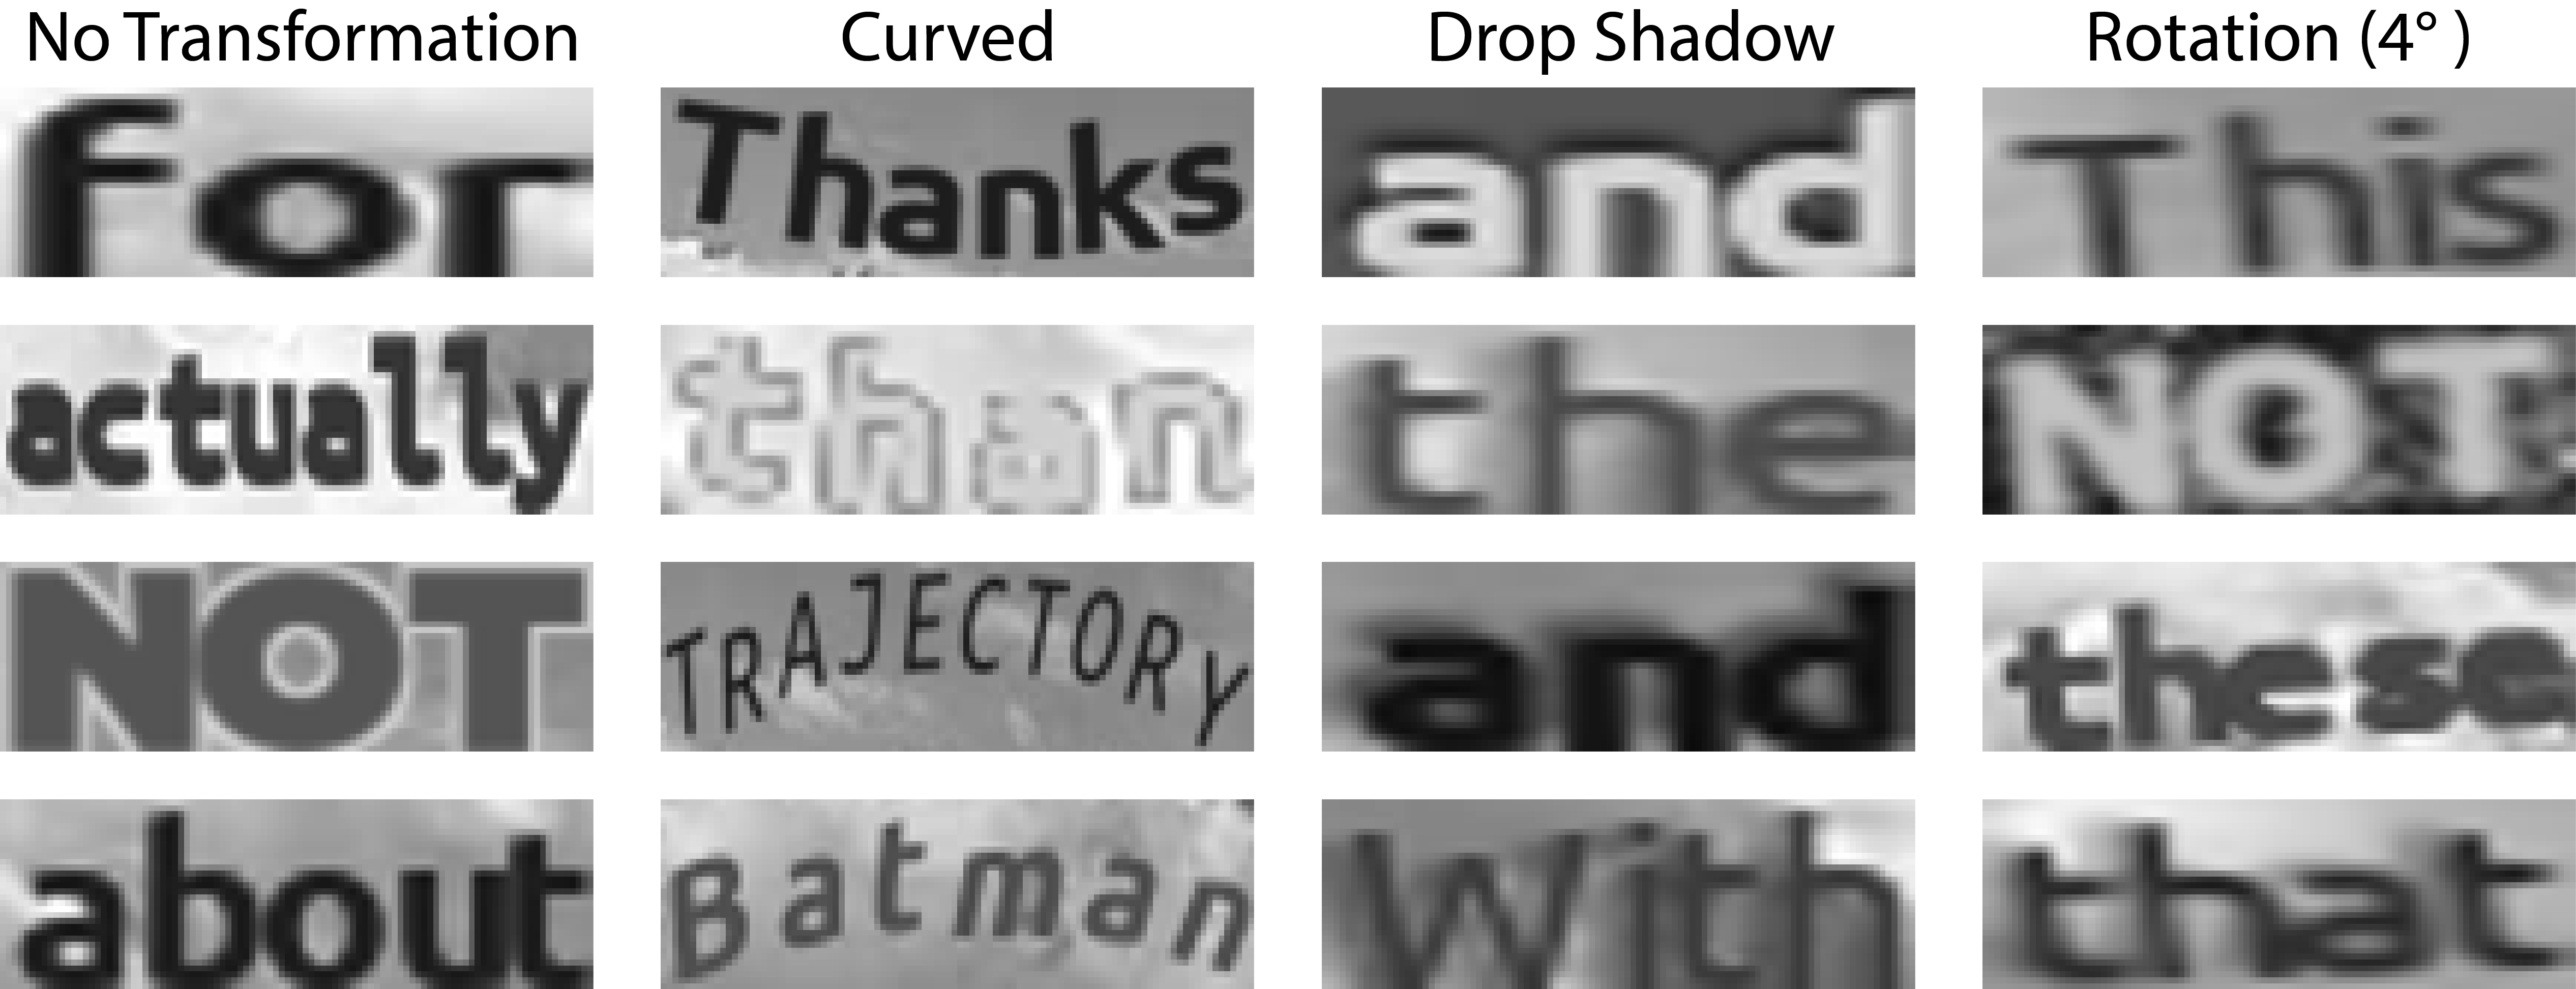
\includegraphics[width=\columnwidth]{Figures/synthtext_outputs/synthext_outputs.png}
\caption{Example of generated text from a sample of four different text constraints. The ability to create large test sets with different constraints allows us to compare differences in network activations.}
\label{fig:genText}
\end{figure}


\section{Visualization Pipelines}


\subsection{Standard Visualization techniques applied to the domain of text recognition}
Multiple methods to inspect the learned parameters and internal state exist. For example, learned filters and activations resulting from forward propagation have been visualized \cite{yosinski2015understanding}. The backpropagation visualization calculates derivatives of any unit with respect to any other unit \cite{DBLP:journals/corr/ZeilerF13}. Yosinski compiled these techniques into the Deep Visualization Toolbox \cite{yosinski2015understanding}. After modifying the toolbox and model to be compatible, we visualized the network by seeing its learned filters, activations, and backpropagation.


\subsection{Top Activations Method}
Deep CNNs derive power from implementing chains of simple computations to mimic complex functions. We propose a method which aims to identify a chain of important computations which contribute to the network discriminating between high level features, as opposed to per unit activations. One of the major drawbacks in understanding convolutional layer activations is that the activation map is a matrix, as opposed to a single number, which makes comparing activations across different nodes difficult. Most approaches attempt to resolve this by taking the max element, which we believe may be sub-optimal. We use the frobenius norm of the filter activations to collapse an activation map to a single number, thus helping us compare different nodes. The frobenius norm gives a two fold benefit. Firstly, it takes into account all activations, and secondly it amplifies the importance of outliers, which in principle acts like a more relaxed version of picking the max element. 

For a particular class of input images, the activations for all filters are recorded, and the frobenius norm for each map is calculated. Each node is given an ID and for each input image, the top N nodes with the maximum norm are extracted per layer. We log these top nodes for all input images, and then report the M nodes per layer that occur most often across all input images belonging to one class. These M nodes then define the subnetwork which contributed the most to the specific input class. After trying different values for N and M, we found that best resolution and separation was found at N=10 nodes per layer, and M=15 nodes per subnetwork. The results elaborate on our selection criteria in greater detail.

\begin{figure}
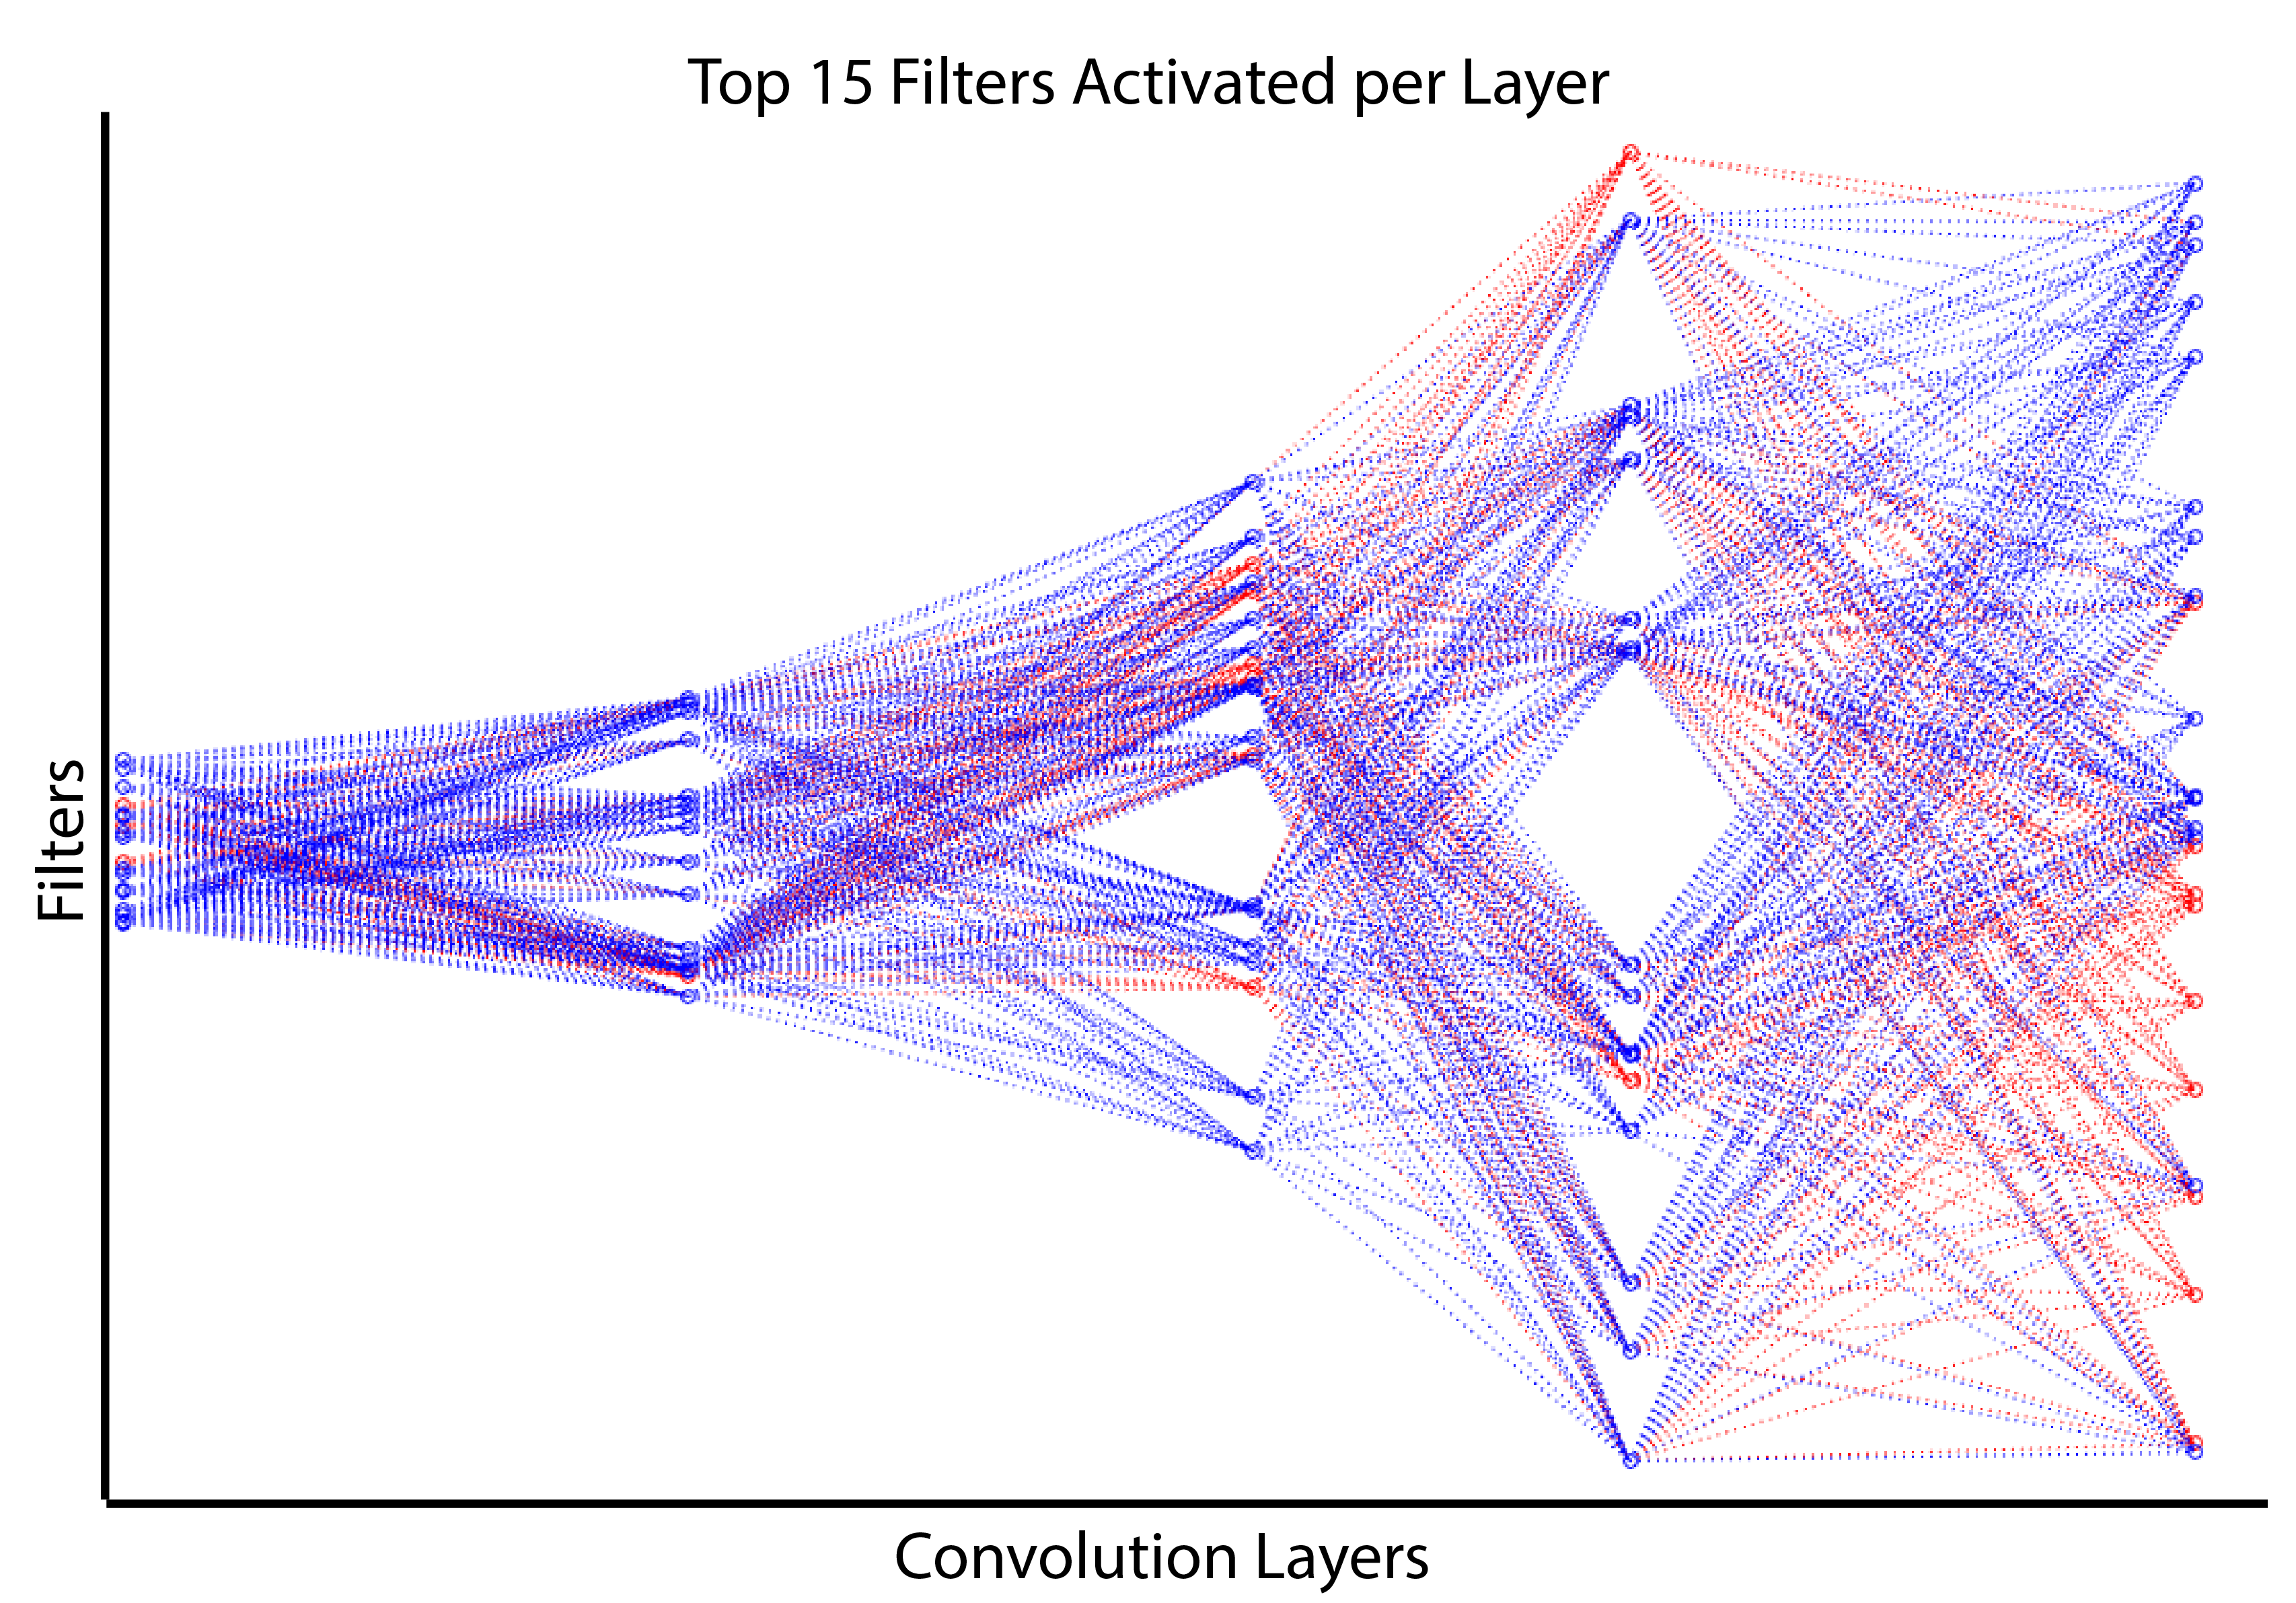
\includegraphics[width=\columnwidth]{Figures/max_activations/max_activations-01.png}
\caption{Resulting subnetworks from the top activations methods. The red nodes and lines correspond to the top filters as activated by images of the letter 't'; likewise for blue, the letter 'o'. Early layers show substantial overlap, but differentiation occurs in later layers.}
\label{fig:activationgraph}
\end{figure}


\subsection{Activation Signature through difference maps} \label{sec:subnetwork}
\begin{figure*}
\centering
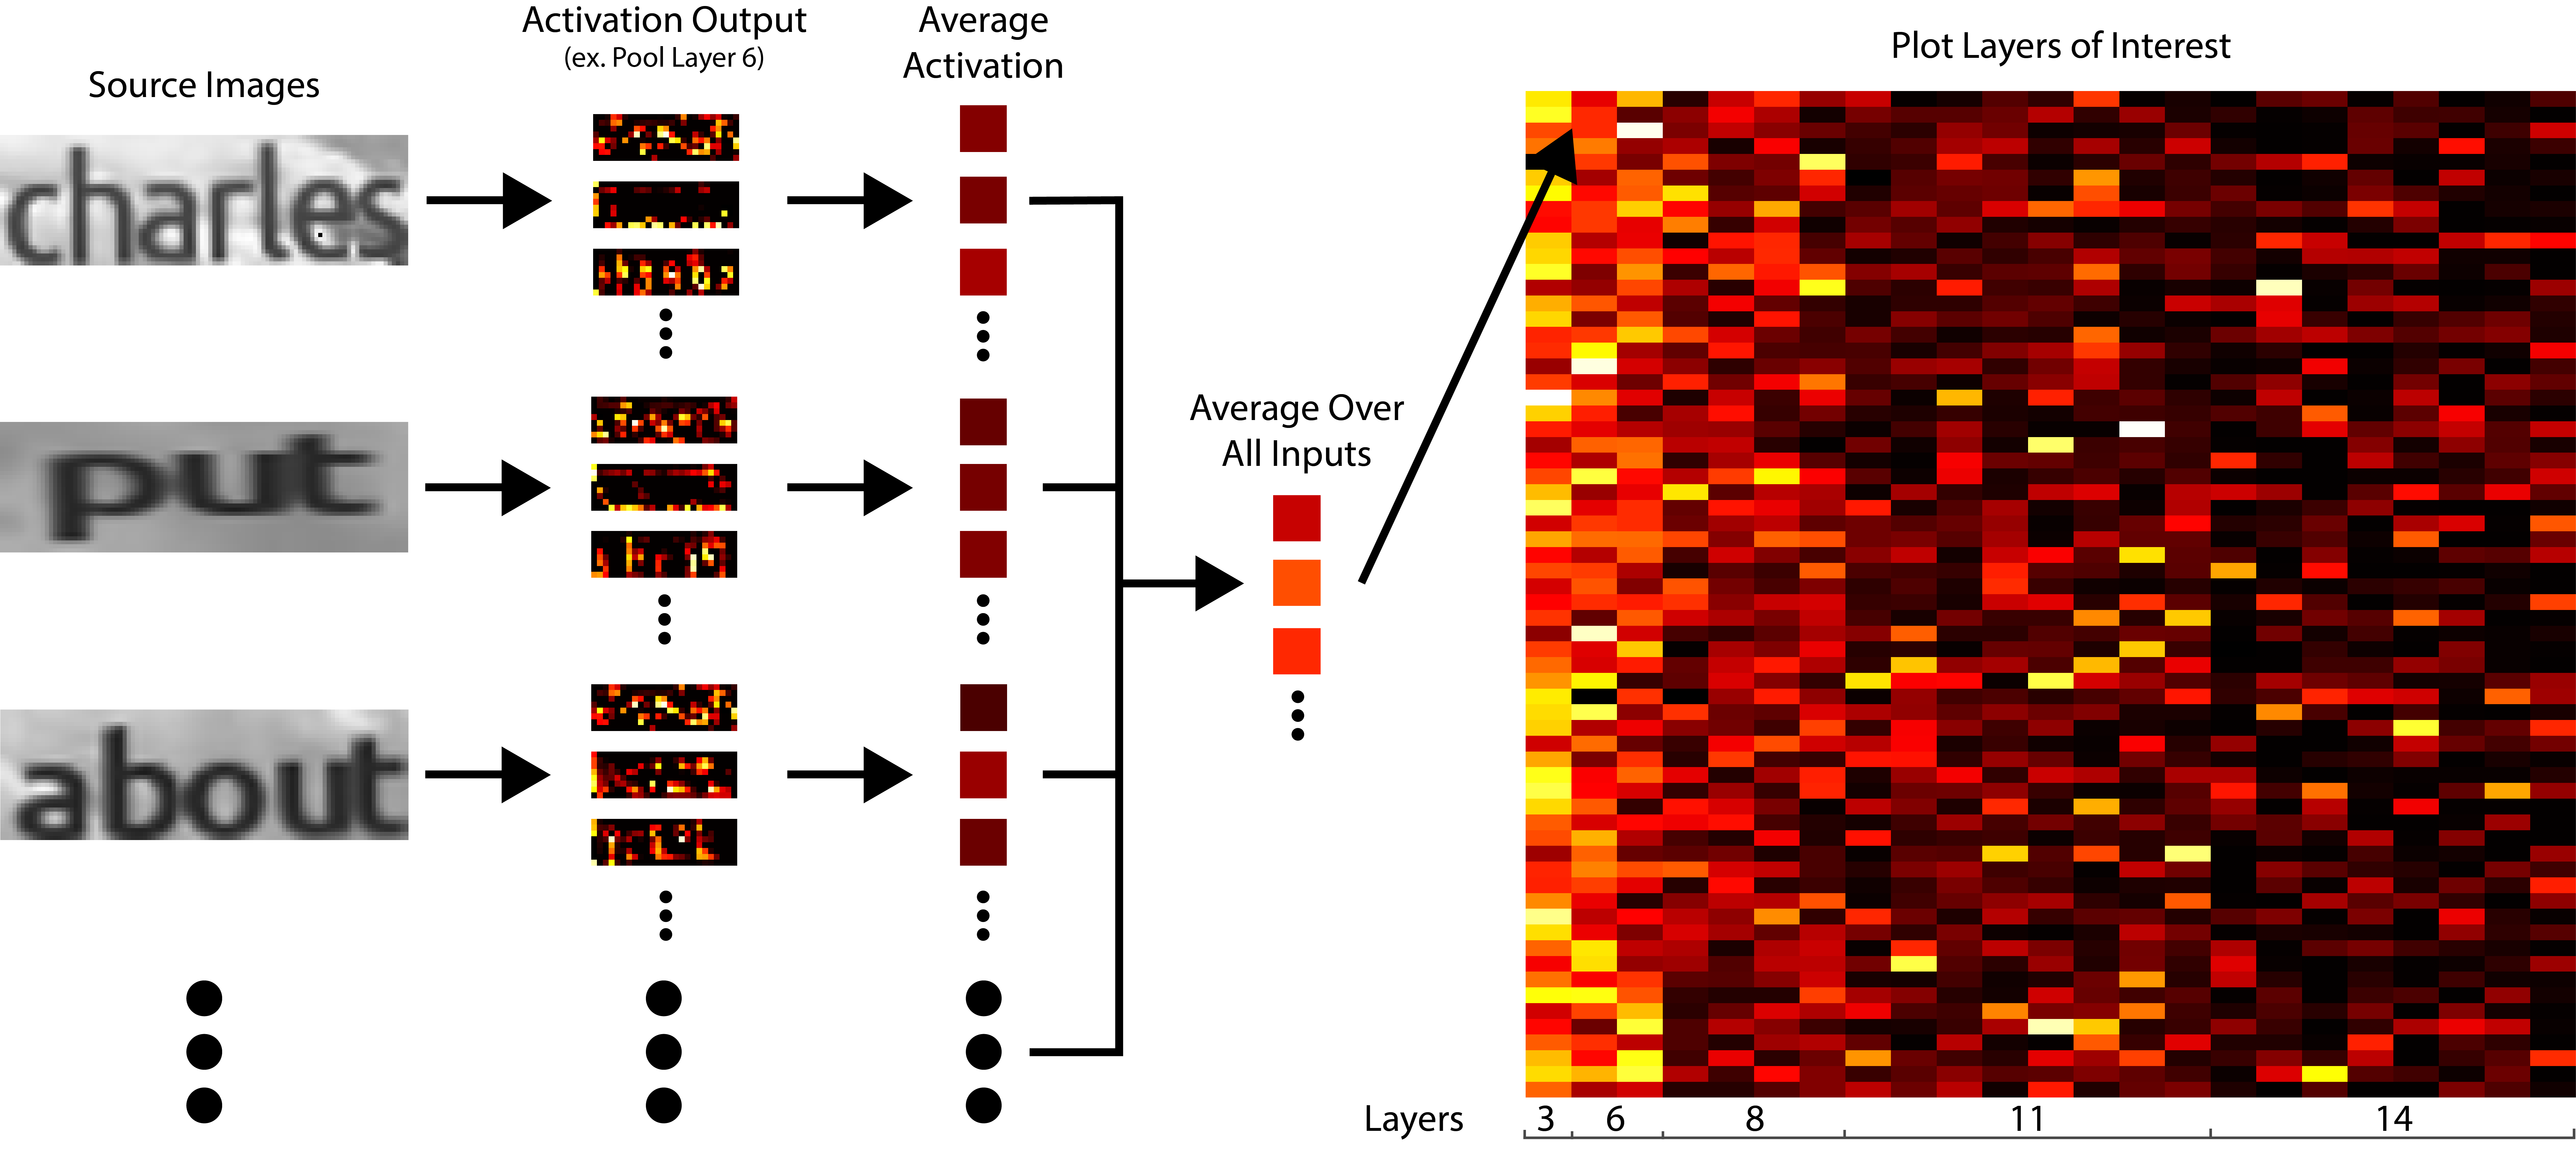
\includegraphics[width=1\textwidth]{Figures/activations_map_overview/act_map_overview-01.png}
\caption{Illustration describing how the activation maps are created. First $\sim$1000 text images are fed through the network. The activation outputs are recorded for each layer. Each individual filter activation is averaged. These averaged activation are then averaged over all of the source images and plotted on a 2D grid. Since the number of filters per layer varies, we give additional columns to layers with more filters (For example layer 8 has 4 columns). The layers chosen are either RELU or pooling operations and occur prior to either a convolution or fully connected layer.}
\label{fig:subvis}
\end{figure*}


\begin{figure}
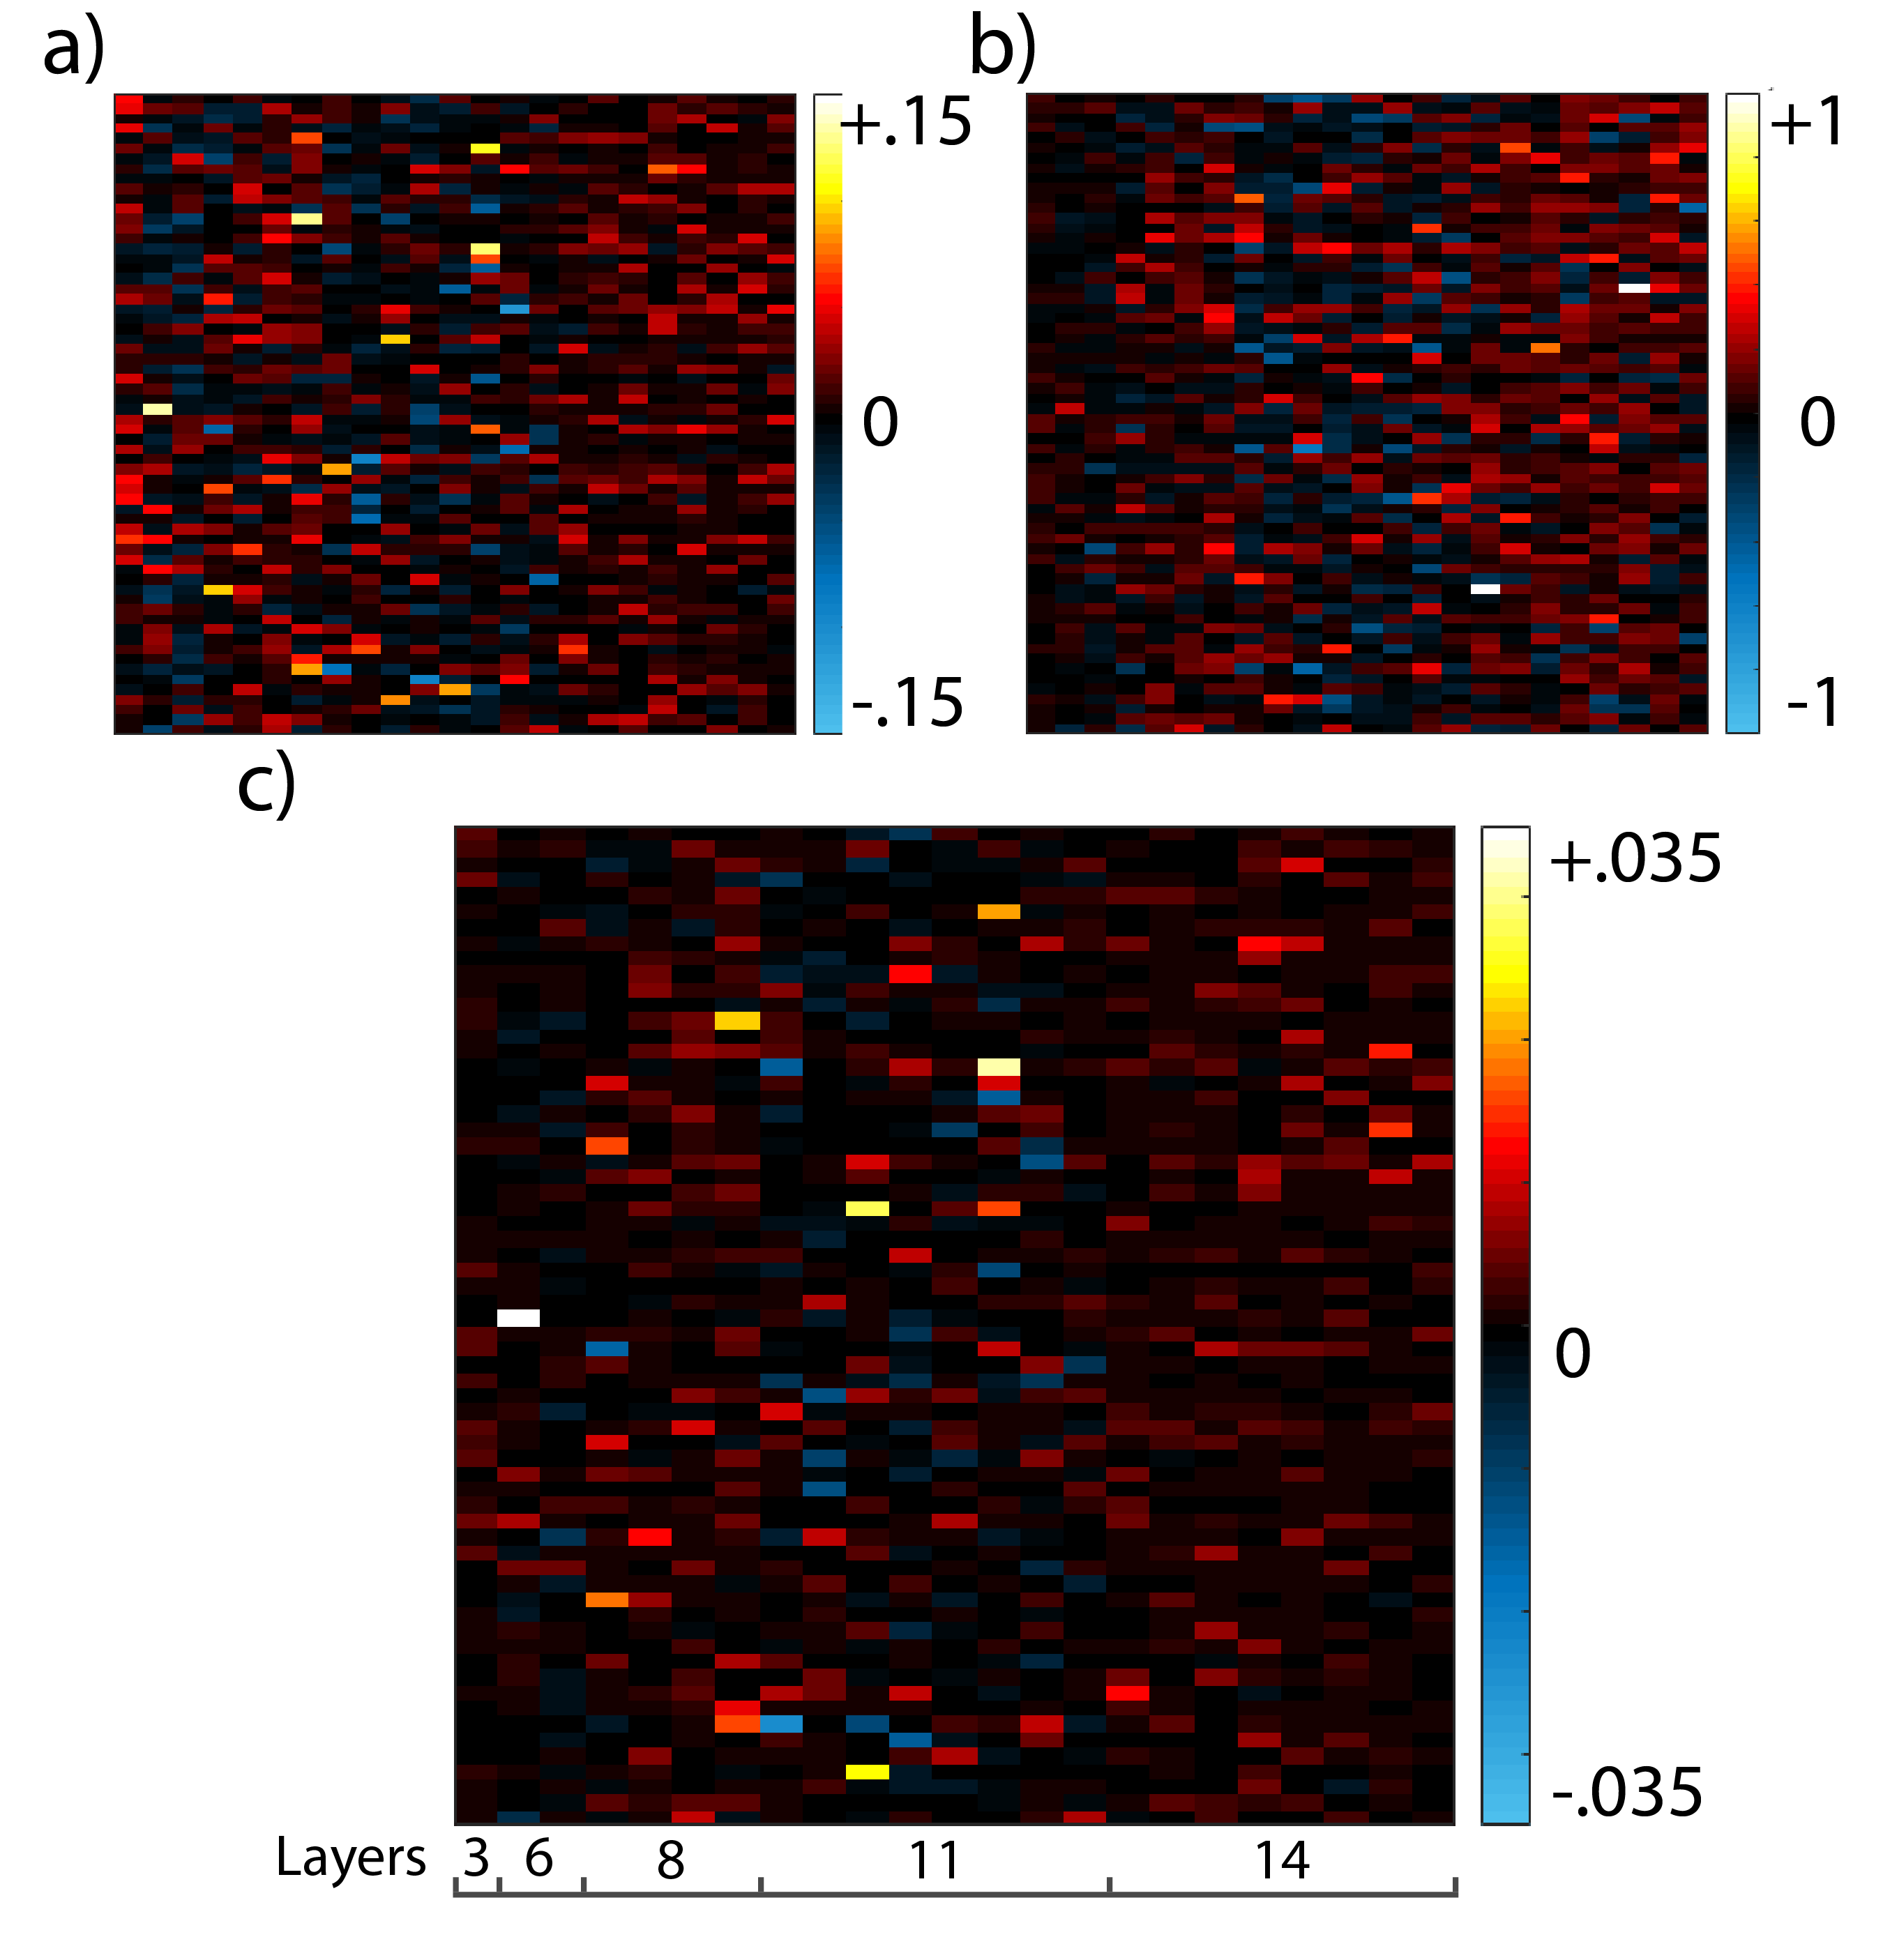
\includegraphics[width=\columnwidth]{Figures/diff_comparisons/diff_comparison-01.png}
\caption{Generated difference maps for comparing a test set  with drop shadows $V_1$, and without $V_0$. a) First we look at the simple case of $V_1-V_0$. We note the differences are spread over the network. b) To get an example of the relative impact we use $\frac{V_1-V_0}{V_0}$. Activity shifts to the later layers as they have lower initial activation values so their relative difference is greater. c) $\frac{V_1-V_0}{V_0}*|V_1-V_0|$ A combination of method a and method b that emphasizes outliers.}
\label{fig:diffmethods}
\end{figure}


We propose a method to isolate subnetworks by using activations. Similar to how a neurologist would map the brain \cite{friston1998event}, we probe the network with different datasets and observe how the network reacts. Our method focuses on the amount of activation at each node. As an example assume we are interested in finding a subnetwork associated with a specific transformation. First two specialized synthetic datasets are generated as described in section \ref{sec:synthtext}. In this case one dataset does not have the transformation and the other does. The datasets are fed through the network and the activations are recorded and visualized. To visualize the activations, each filter output is averaged. Each of these resulting values are averaged over all of the test inputs. Finally the resulting values are mapped on a 2D plane as shown in Fig. \ref{fig:subvis}. The visualized layers included are either the RELU or pooling layer and occur before either convolution layers or fully connected layers. This is because visualizing activation values that are subsequently dropped (due to RELU and pooling operations) provides little value. Two maps are created, $V_0$ and $V_1$, for the dataset with and without the transformations. Comparisons between $V_0$ and $V_1$ can be used to get and idea about how the network reacts to the transformation. Different comparison metrics are explored in Fig. \ref{fig:diffmethods}. We found the following metric the most valuable for visualizations as it emphasized relative difference while maintaining the sign of the value:
\begin{equation} \label{eq:1}
\frac{V_0-V_1}{V_0} * |V_0-V_1|
\end{equation}


This method attempts to visualize the structure of the network rather than node specific operations as is typically done. The structure view provides an abstraction that is useful when discussing operations that are difficult to visualize. For example, it is difficult and uninformative to visualize transformations (rotation, scale, translation, etc). However understanding which parts of the network are active during different transformations can be informative. This information can be used for network pruning and other architecture optimizations. To do these network operations efficiently would require constructing the network differently. We leave this analysis to a future study.

\section{Results}

\begin{figure}
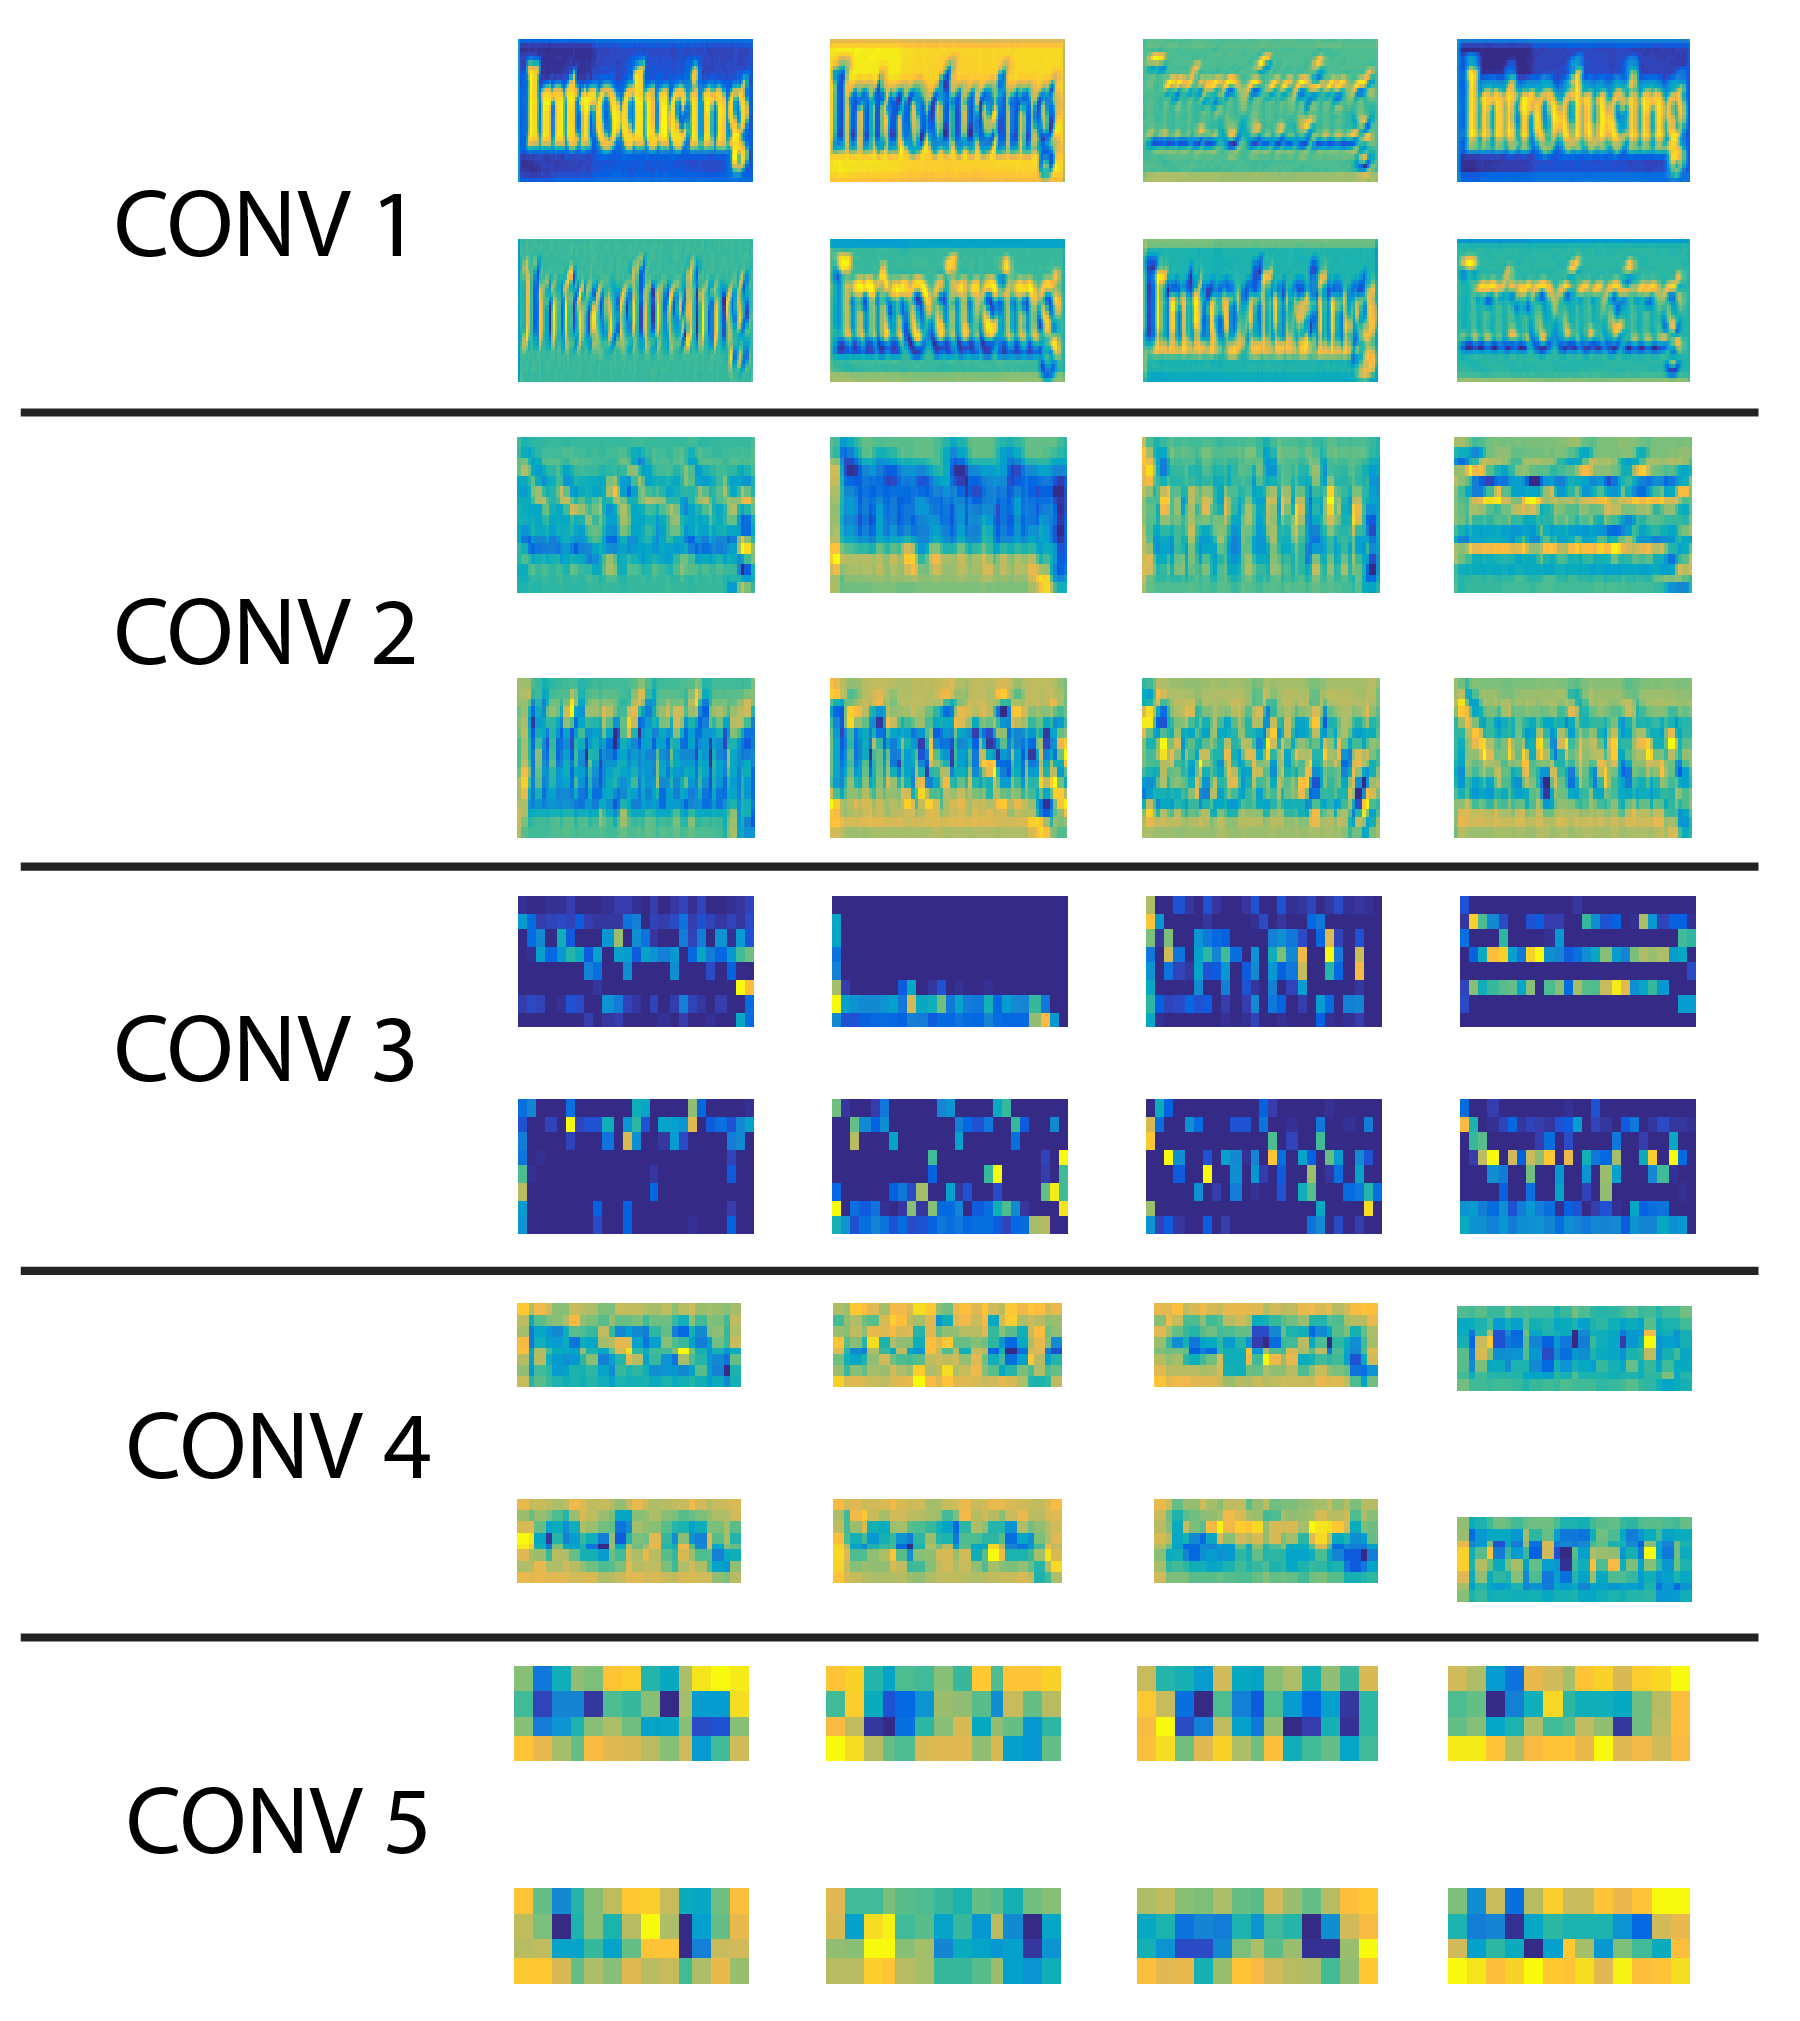
\includegraphics[width=\columnwidth]{Figures/activation_vis/activation_vis-01.png}
\caption{Visualizing activations of different filters}
\label{fig:deepvis}
\end{figure}

\begin{figure}
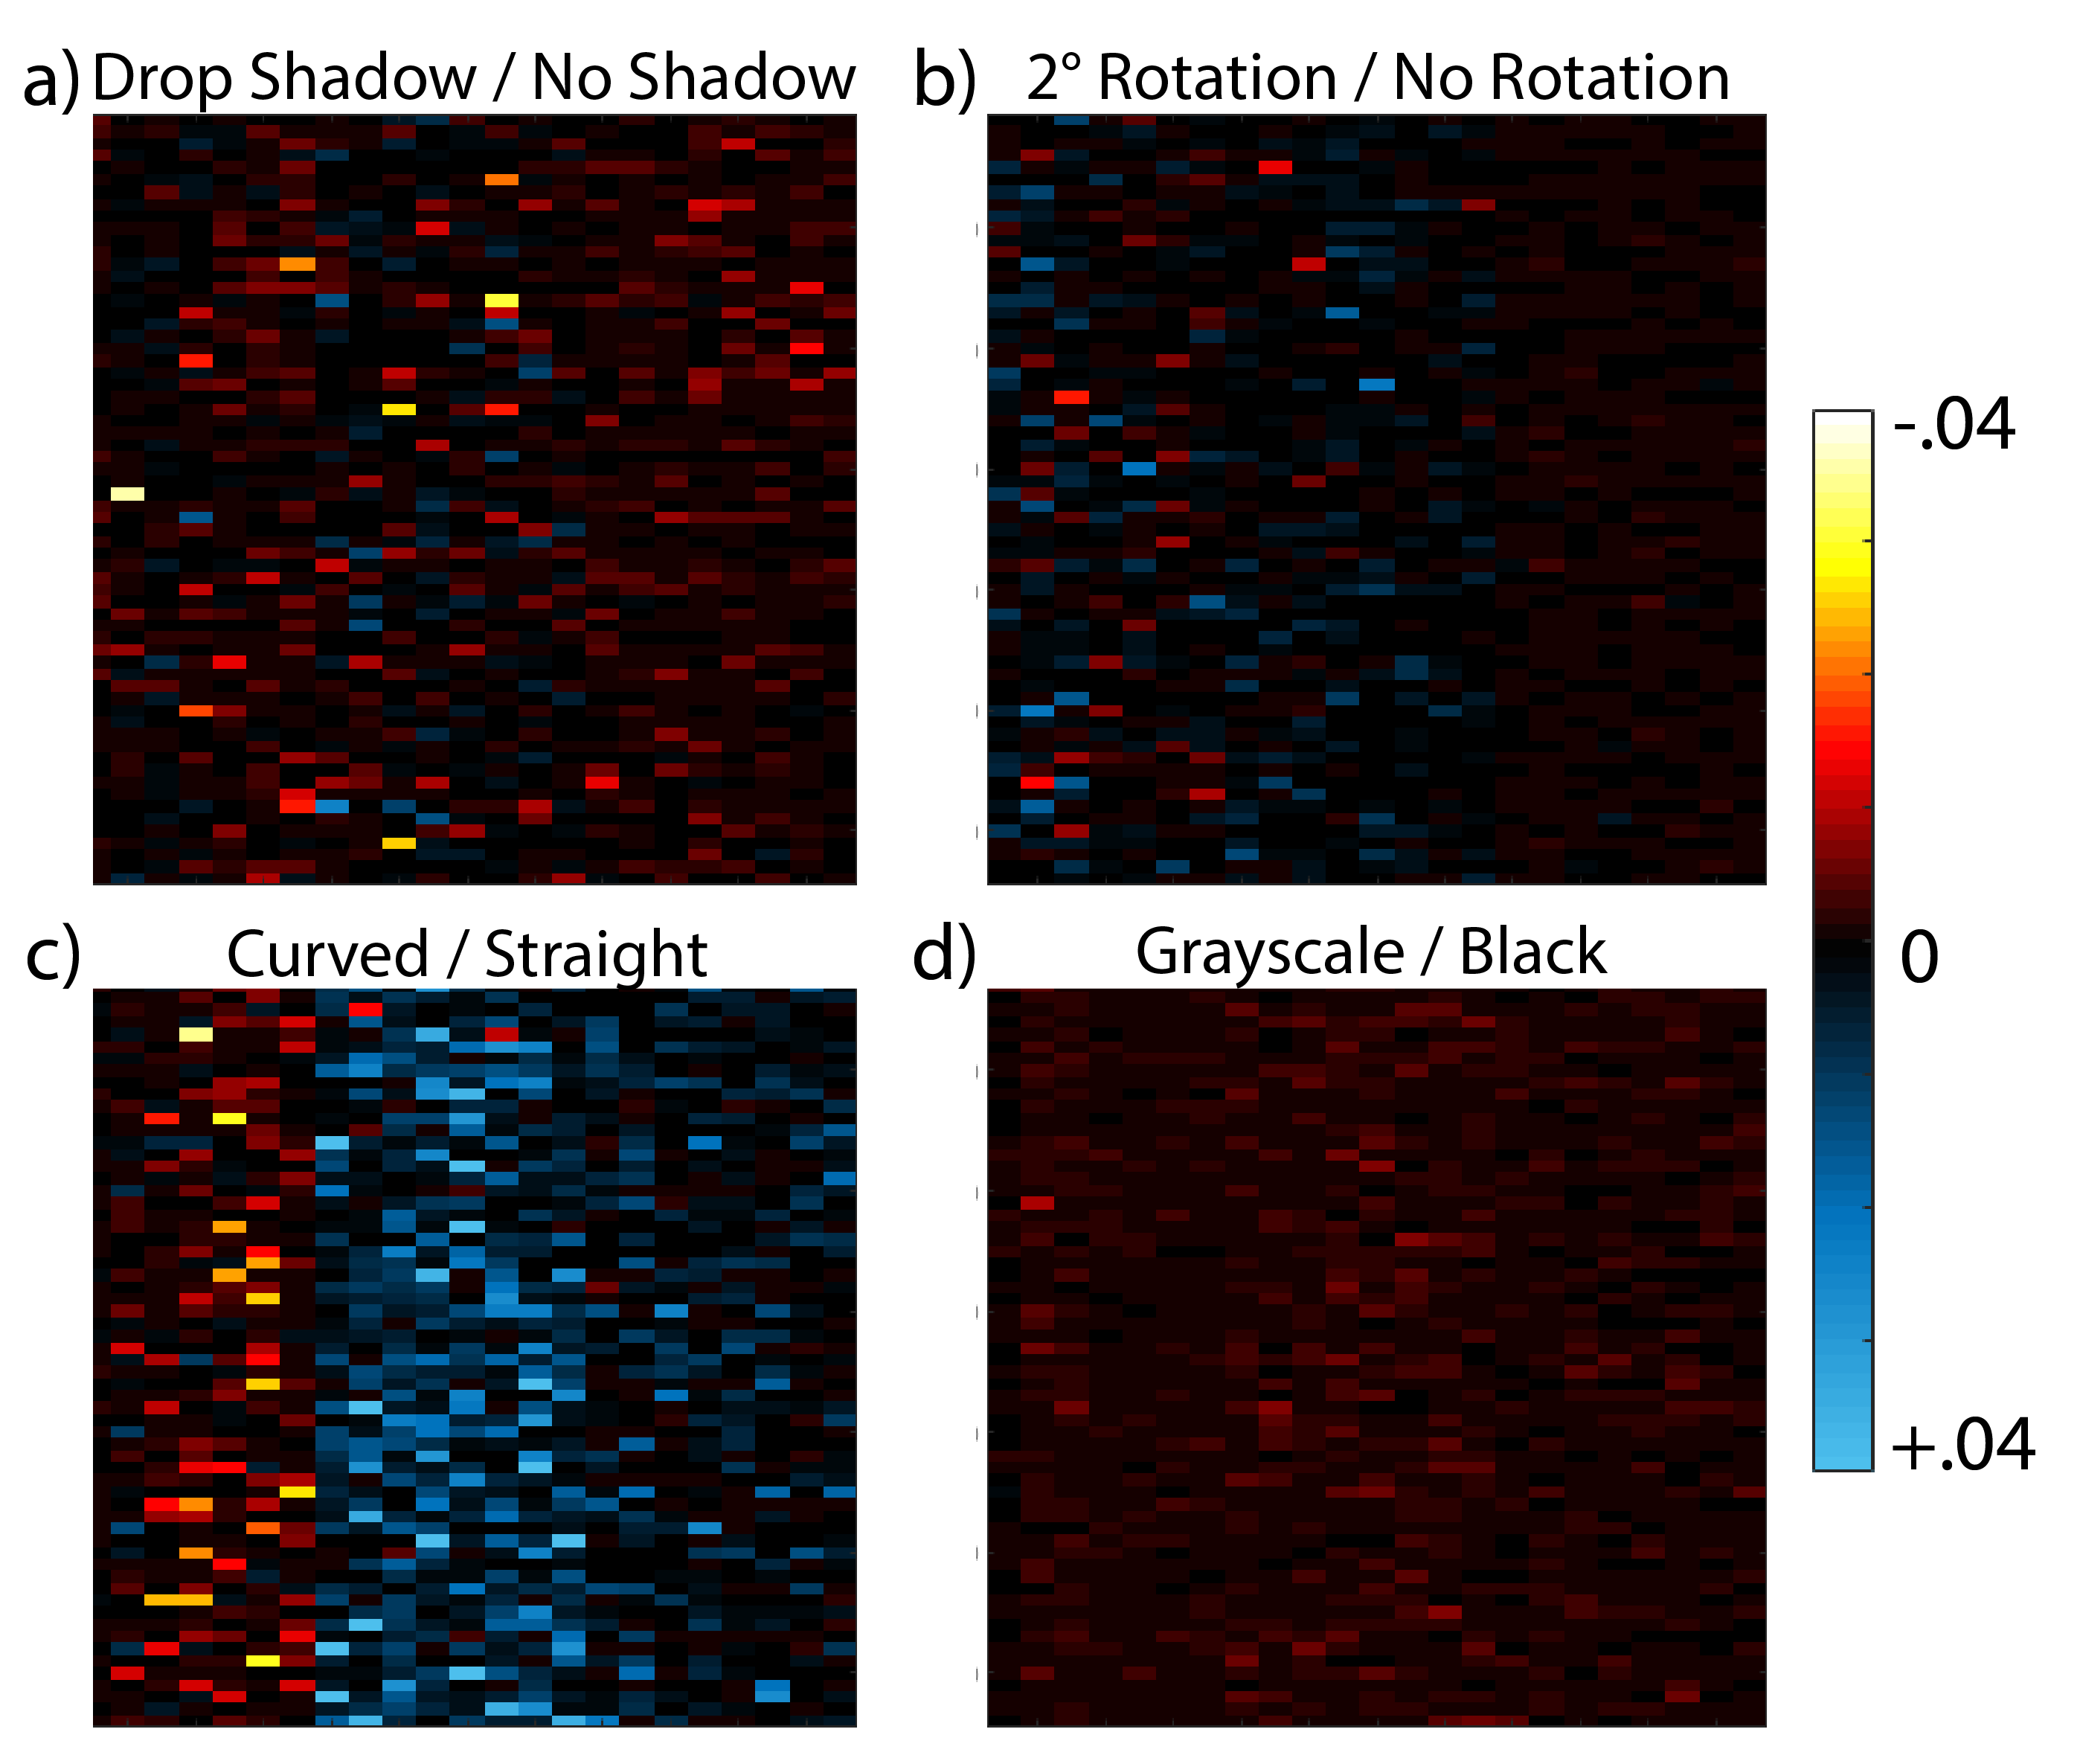
\includegraphics[width=\columnwidth]{Figures/diff_examples/diff_examples-01.png}
\caption{A set of generated difference maps using Eq. \ref{eq:1}. a) Comparing text with drop shadows to text without. We find that there are a few nodes that are effected more than the others. b) Comparing text with a rotation to text without. We note that the difference map is similar to the shadow comparison however the activations are not as strong. c) Comparing curved text with straight text. We note a sharp distinction between the earlier layers and the later layers. It appears that the earlier layers more strongly activated by the curved text whereas the later layers react strongly towards the straight text. d) Comparing text that contains gray scale values to text that is all black. We note the gray scale text increases the activation throughout the network.}
\label{fig:diffexamples}
\end{figure}

\subsection{Standard Visualization Techniques}
To better understand the functioning of the text detector, we ported it over to Caffe from Matconvnet, and then used a toolkit provided by \cite{yosinski2015understanding} to visualize the filers and their activations for different kinds of input images. Also, we visualized the activations ourselves in MATLAB and eyeballed ther results to make sense of how the network works, as shown in Fig. \ref{fig:deepvis}

We found that we can trace the process of text recognition through the layers, breaking it down into high level tasks. Initial layers of the network roughly identified the horizontal and vertical edges in the words. As we move further, the word is no longer visible, but filter activations are localized in groups of high density. This was intriguing, and is one of the problems we will be following up in our future work. As we moved towards the end of the network, activations became more sparse and less localized. Activation maps contained 3-4 very high activations, and the rest were usually very low. This prompted us to use a metric other than maximum to compare different activation maps, and we moved to a frobenius norm as explained earlier. 

Finally, towards the last layers, the activations were highly sparse, and most activations had been forced down to zero - most filters were dead/not contributing. This was expected, and motivated us to try and identify subnetworks that map to learning high level features in the input images. The next two sections show the results for these methods trying to identify useful substructures in the network.

\subsection{Top Activations Method}
Fig. \ref{fig:subvis} visualizes the top activations for the red 't' class and the blue 'o' class. Early layers show substantial overlap, but differentiation occurs in later layers. This corresponds to how the network identifies features from general to specific -- lower layers would detect simple features like edges and whitespace, which is required for all characters, whereas higher layers would specialize into shape finders, and ultimately letter categorizers. 

\subsection{Difference Maps}
Using Eq. \ref{eq:1} as our difference metric, we create four activation signatures for different text transformations; refer to Fig. \ref{fig:diffexamples}. Specific transformations were chosen that are hard to visualize using traditional techniques. The tests included comparing shadows, rotations, curviness, and color. Interestingly structurally different signatures for the different transformations emerged. For example, inspecting curved text compared to straight text we see a boundary between the first layers and the last layers. This allows us to localize parts of the network to particular tasks. The shadow comparison and the rotation comparison do no appear to be localized to specific layers. However it does appear that some nodes are more important than others. Finally our color test shows that increasing the variability in color input increases the activation across the layers.




%-------------------------------------------------------------------------
\section{Discussion}
Identifying sub-networks can prove to be extremely useful at different steps in CNN training and deployment. It can help decide leaner network architecture depending upon known invariants in the training dataset, and prune existing networks without reducing accuracy over certain datasets. Furthermore, it can, in principle, facilitate a plug-and-play use of sub-networks for transfer learning to new domains akin to the fine-tuning approach which is gaining popularity in the computer vision community.

Top Activations:
Having roughly identified two different subnetworks, one for the 't' class and one for the 'o' class, the top activations method seems promising. Further work includes attempting the method for all input classes, as well as developing a metric to judge the separability of the subnetworks that have been identified. In addition, the parameters N and M are specific to this model - a heuristic or a way to automatically select these parameters is a promising line of investigation.

Activation Signatures:
Different signatures for different transformations were observed. Further work include using these signatures to inform architecture choices. For example we note the layer dependence in the curved transformation. Network pruning may also be possible as we found specific filters that were activated strongly with the shadow and rotation transformations. Activation signatures provide a new analysis tool to help shed light on these increasingly complex networks. 

%-------------------------------------------------------------------------


%-------------------------------------------------------------------------
\subsection{Conclusion}
Traditional per-unit visualization tools like the Deep Visualization Toolbox \cite{yosinski2015understanding} show that the text detection network operates similar to an object or scene detector. To get a more zoomed out perspective of the information flow, we proposed two new general purpose techniques for identifying highly activated sub-networks. The Top Activations method attempts to capture the essence of the chained convolutions which make neural networks so successful. The Activation Signature method visualizes the differences in activations corresponding certain input transformations. This helps identify an activation signature for each transformation. These subnetwork identification methods may prove to be useful in debugging and optimizing network architectures as they may help map high level features of the image to regions in the network. Future work includes continuing searching for exemplar subnetworks corresponding to particular high level tasks.


%------------------------------------------------------------------------
\subsection{Contributions}
Our project can be roughly divided into 5 parts, and we started with an equitable distribution of work among the three of us. The five parts are: 
\begin{enumerate}
\item Setting up models and porting them to make sure systems run
\item Standard visualization techniques used in literature, Deep visualization toolbox
\item Top Activations Method, Identifying subnetworks - the first proposed technique
\item Synthetic text generation pipeline and Activations Signature Method to get Difference Maps - the second proposed technique
\item Presentation and Paper
\end{enumerate}

Spandan Madan and Shantanu Jain worked together on Parts 1,2 and 3. Part 4 was done by Matthew Tancik, and all three worked together on Part 5. All work was discussed periodically by all three members to make sure we keep on track and we all guided each other in terms of understanding how things are working. All in all, it was a team effort.


{\small
\bibliographystyle{ieee}
\bibliography{egbib}
}


\end{document}








